\documentclass[journal,12pt,twocolumn]{IEEEtran}

\usepackage{enumitem}
\usepackage{amsmath}
\usepackage{amssymb}
\usepackage{gensymb}
\usepackage{graphicx}
\usepackage{txfonts}         
\usepackage{listings}
\usepackage{lstautogobble}
\usepackage{mathtools}
\usepackage{bm}
\usepackage{hyperref}
\usepackage{polynom}
\usepackage{capt-of}
\newcommand{\solution}{\noindent \textbf{Solution: }}
\providecommand{\pr}[1]{\ensuremath{\Pr\left(#1\right)}}
\providecommand{\brak}[1]{\ensuremath{\left(#1\right)}}
\providecommand{\cbrak}[1]{\ensuremath{\left\{#1\right\}}}
\providecommand{\sbrak}[1]{\ensuremath{\left[#1\right]}}
\providecommand{\mean}[1]{E\left[ #1 \right]}
\providecommand{\var}[1]{\mathrm{Var}\left[ #1 \right]}
\providecommand{\der}[1]{\mathrm{d} #1}
\providecommand{\gauss}[2]{\mathcal{N}\ensuremath{\left(#1,#2\right)}}
\providecommand{\mbf}{\mathbf}
\providecommand{\abs}[1]{\left\vert#1\right\vert}
\providecommand{\norm}[1]{\left\lVert#1\right\rVert}
\providecommand{\z}[1]{{\mathcal{Z}}\{#1\}}
\providecommand{\ztrans}{\overset{\mathcal{Z}}{ \rightleftharpoons}}
\providecommand{\system}[1]{\overset{\mathcal{#1}}{ \longleftrightarrow}}
\providecommand{\laplaceinv}[1]{{\mathcal{L}^{-1}\ensuremath{\left[#1\right]}}}
\providecommand{\parder}[2]{\frac{\partial}{\partial #2} \brak{#1}}

\let\StandardTheFigure\thefigure
\let\vec\mathbf

\numberwithin{equation}{section}
\renewcommand{\thefigure}{\theenumi}
\renewcommand\thesection{\arabic{section}}

\newcommand{\myvec}[1]{\ensuremath{\begin{pmatrix}#1\end{pmatrix}}}
\newcommand{\mydet}[1]{\ensuremath{\begin{vmatrix}#1\end{vmatrix}}}
\newcommand{\define}{\stackrel{\triangle}{=}}

\DeclareMathOperator*{\argmin}{arg\,min}
\DeclareMathOperator*{\argmax}{arg\,max}


\lstset {
	frame=single, 
	breaklines=true,
	columns=fullflexible,
	autogobble=true
}             
   


\begin{document}
                             
\title{ Digital Signal Processing \\ \Large EE3900 \\ \vspace*{12pt} \textbf{Fourier Series}}
\author{I Sai Pradeep\\ \normalsize AI21BTECH11013 \\ \vspace*{20pt} \normalsize \today}
 \maketitle 
 \tableofcontents
 \begin{abstract}
    This manual provides a simple introduction to Fourier Series
    \end{abstract}
    \section{Periodic Function}
    Let 
    \begin{align}
        x(t) &= A_0\abs{\sin\brak{2\pi f_0 t}}
        \label{eq:x(t)}
    \end{align}
    \begin{enumerate}[label=\thesection.\arabic*
    ,ref=\thesection.\theenumi]
    \item Plot $x(t)$.\\
    \solution 
    \begin{lstlisting}
wget https://github.com/Pradeep8802/EE3900-Digital-Signal-Processing/blob/main/charger/codes/1.1.py
    \end{lstlisting}
    \begin{figure}[!ht]
			\centering
			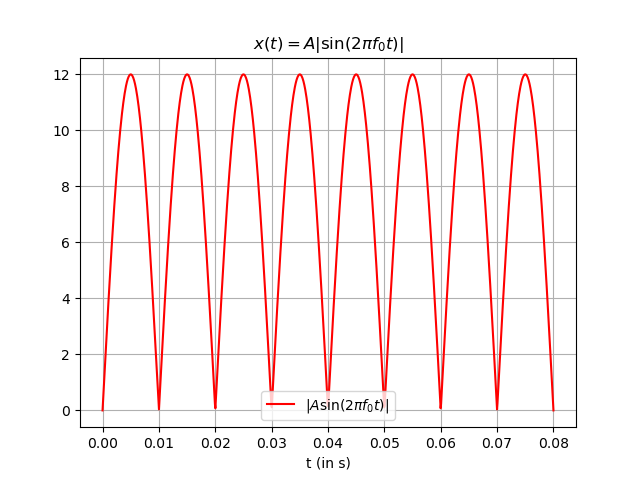
\includegraphics[width=\columnwidth]{./figs/1.1.png}
			\caption{}
			%\label{fig:ckt}
\end{figure}
    \item Show that $x(t)$ is periodic and find its period.
    \solution 
    A signal $x(t)$ is said to be periodic with fundamental period $T$ if
    \begin{align}
    \label{eq:peroidic}
    x(t+nT)=x(t) \forall n \in \mathbb{Z}
    \end{align}
Let $T$ be fundamental period of $x(t)$. Comparing \eqref{eq:peroidic} and \eqref{eq:x(t)}, we get
	\begin{align}
A_0\abs{\sin\brak{2\pi f_0 t}}&=A_0\abs{\sin\brak{2\pi f_0 (t+T)}}\\
\abs{\sin\brak{2\pi f_0 t}}&=\abs{\sin\brak{2\pi f_0 (t+T)}}\\
\abs{\sin\brak{2\pi f_0 t}}&=\abs{\sin\brak{2\pi f_0 t+2\pi f_0 T)}}
	\end{align}
As $|sin\theta|$ is periodic with fundamental period $F=\pi$, Hence,
    \begin{align}
\abs{\sin\brak{t}}=\abs{\sin\brak{t+F)}}
\end{align}
Hence,$2\pi f_0  T=\pi$, therefore, fundamental period($T$) is 
\begin{align}
\label{eq:ftp}
T=\frac{\pi}{2 \pi f_0}=\frac{1}{2f_0}
    \end{align}
    \end{enumerate}
    \section{Fourier Series}
    Consider $A_0 =12$ and $f_0 = 50$ for all numerical calculations.
    \begin{enumerate}[label=\thesection.\arabic*,ref=\thesection.\theenumi]
    \item If
    %\cite{proakis_dsp}
    \begin{align}
        x(t) = \sum_{k = -\infty}^{\infty}c_ke^{j2\pi kf_0 t}
    \label{eq:one-Z-complex}
    \end{align}
    show that 
    \begin{align}
        c_k = f_0\int_{-\frac{1}{2f_0}}^{\frac{1}{2f_0}}x(t)e^{-j2\pi kf_0 t}\, dt
    \label{eq:one-Z}
    \end{align}
    \solution 
    From \eqref{eq:one-Z-complex},
    \begin{align}
    	\label{eq:sum}
            x(t) = \sum_{k = -\infty}^{\infty}c_ke^{j2\pi kf_0 t}
    \end{align}
    Mulitply $e^{-j2\pi lf_0 t}$ on both sides of \eqref{eq:sum}, we get,
    \begin{align}
    	\label{eq:a}
    x(t)e^{-j2\pi lf_0 t}=\sum_{k = -\infty}^{\infty}c_ke^{j2\pi kf_0 t}e^{-j2\pi lf_0 t}
    \end{align}
    Integrating \eqref{eq:a} w.r.t. $t$ from $-T$ to $T$, and $T=\frac{1}{f_0}$, we get,\\
    \begin{align}
    	\label{eq:d}
    \int_{-\frac{1}{2f_0}}^{\frac{1}{2f_0}}x(t)e^{-j2\pi kf_0 t}\, dt&=\int_{-\frac{1}{2f_0}}^{\frac{1}{2f_0}}\sum_{k = -\infty}^{\infty}c_ke^{j2\pi \brak{k-l}f_0 t}\,dt\\
    &=\sum_{k = -\infty}^{\infty}c_k\int_{-\frac{1}{2f_0}}^{\frac{1}{2f_0}}e^{j2\pi \brak{k-l}f_0 t}\,dt
    \end{align}
Consider the following cases.\\
case-1:$k=l$
\begin{align}
	\int_{-\frac{1}{2f_0}}^{\frac{1}{2f_0}}e^{j2\pi \brak{k-l}f_0 t}\,dt&=\int_{-\frac{1}{2f_0}}^{\frac{1}{2f_0}}e^{0}\,dt\\
	&=\int_{-\frac{1}{2f_0}}^{\frac{1}{2f_0}} 1 \,dt
\end{align}
case-2: $k \neq l$ \\
Let $n=f_0(k-l)$, here $n \in \mathbb{Z}$
\begin{align}
	\label{eq:b}
\int_{-\frac{1}{2f_0}}^{\frac{1}{2f_0}}e^{j2\pi \brak{k-l}f_0 t}\,dt&=\int_{-\frac{1}{2f_0}}^{\frac{1}{2f_0}}e^{2n\pi}\,dt	
\end{align}
Here, $2n\pi T=2f_0(k-l)T\pi$, and $2n\pi T=(k-l)\pi$
\begin{align}
\int_{-\frac{1}{2f_0}}^{\frac{1}{2f_0}}e^{j2n\pi}\,dt&=\int_{-\frac{1}{2f_0}}^{\frac{1}{2f_0}}1\,dt\\&=\int_{-\frac{1}{2f_0}}^{\frac{1}{2f_0}}\cos(2n\pi)+j\sin(2n\pi) \,dt
\end{align}
\begin{align}
\int_{-\frac{1}{2f_0}}^{\frac{1}{2f_0}}e^{j2n\pi}\,dt&=
-\sin(2n\pi t)\bigg|_{-\frac{1}{2f_0}}^{\frac{1}{2f_0}}\\&+j\cos(2n\pi t)\bigg|_{-\frac{1}{2f_0}}^{\frac{1}{2f_0}}\\
&=-\sin(2n\pi t)\bigg|_{-\frac{1}{2f_0}}^{\frac{1}{2f_0}}\\&+j\cos(2n\pi t)\bigg|_{-\frac{1}{2f_0}}^{\frac{1}{2f_0}}\\
&=-\sin(2n\pi t)\bigg|_{-\frac{1}{2f_0}}^{\frac{1}{2f_0}}\\&+j\cos(2n\pi t)\bigg|_{-\frac{1}{2f_0}}^{\frac{1}{2f_0}}\\
\label{eq:c}\\
&=-\sin((k-l)\pi)+\sin(-(k-l)\pi)\\&+j\cos((k-l)\pi)-j\cos(-(k-l)\pi)\\
\end{align}
Since $k-l \in \mathbb{Z}$,$\sin((k-l)\pi)=0$ and $\sin(-(k-l)\pi)=0$, simillarly, as $\cos(\theta)=\cos(-\theta)$, we get $\cos((k-l)\pi)-\cos(-(k-l)\pi)=0$\\
From \eqref{eq:c},
\begin{align}
	\int_{-\frac{1}{2f_0}}^{\frac{1}{2f_0}}e^{j2n\pi}\,dt&=\int_{-\frac{1}{2f_0}}^{\frac{1}{2f_0}}1\,dt\\&=0+j0=0
\end{align}
Hence, we have,
    \begin{align}
\int_{-\frac{1}{2f_0}}^{\frac{1}{2f_0}}e^{j2\pi \brak{k-l}f_0 t}\,dt=
         \begin{cases}
0 & k\neq l
\\
 \int_{-\frac{1}{2f_0}}^{\frac{1}{2f_0}}1\,dt& k=l
\end{cases}
    \end{align}
From \eqref{eq:d},
    \begin{align}
    	\int_{-\frac{1}{2f_0}}^{\frac{1}{2f_0}}x(t)e^{-j2\pi kf_0 t}\, dt&=\sum_{k = -\infty}^{\infty}c_k\int_{-\frac{1}{2f_0}}^{\frac{1}{2f_0}}e^{j2\pi \brak{k-l}f_0 t}\,dt\\
    	&=c_k \times \int_{-\frac{1}{2f_0}}^{\frac{1}{2f_0}}1\,dt
    	\end{align}
    \begin{align}
  c_k &= f_0\int_{-\frac{1}{2f_0}}^{\frac{1}{2f_0}}x(t)e^{-j2\pi kf_0 t}\, dt\\
  \therefore c_k &= \frac{2}{T} \int_{-\frac{1}{T}}^{\frac{1}{T}}x(t)e^{-j2\pi kf_0 t}\, dt
    \end{align}
        \item Find $c_k$ for 
        \eqref{eq:x(t)}\\
        \solution
        We know that,
        \begin{align}
        c_k = 2f_0\int_{0}^{\frac{1}{2f_0}}x(t)e^{- j2 \pi kf_0 t}\, dt
        \end{align}
when $t \in \bigg( 0,\frac{1}{2f_0}\bigg)$, $x(t)=A_0 \sin\brak{2 \pi f_0t}$\\
      \begin{align}
      c_k &= 2f_0\int_{0}^{\frac{1}{2f_0}}A_0 \brak{\frac{e^{j2\pi f_0t}-e^{-j 2\pi f_0t}}{2j}} e^{- j2 \pi kf_0 t}\,dt\\
      &=A_0f_0\int_{0}^{\frac{1}{2f_0}} \brak{\frac{e^{j2\pi\brak{1-k} f_0t}-e^{j 2\pi\brak{-1-k} f_0t}}{j}}\,dt\\
&=A_0f_0\bigg(\frac{e^{j2\pi\brak{1-k} f_0t}}{-2\pi \brak{1-k}f_0}\bigg|_0^{\frac{1}{2f_0}} \\&- \frac{e^{j2\pi\brak{-1-k} f_0t}}{-2\pi \brak{-1-k}f_0}\bigg|_0^{\frac{1}{2f_0}}\bigg)\\
&=A_0\sbrak{\frac{e^{j\pi\brak{1-k}}-1}{2\pi\brak{k-1}}-\frac{e^{-j\pi\brak{1+k}}-1}{2\pi\brak{k+1}}}
      \end{align}
  Hence,
      \begin{equation}
      \label{eq:ck}
     c_k= \begin{cases}
\frac{2A_0}{\pi\brak{1-k^2}}&k=even
\\
0&k=odd
\end{cases}
      \end{equation}
    \item Verify 
        \eqref{eq:x(t)}
        using python.\\
        \solution 
        \begin{lstlisting}
wget https://github.com/Pradeep8802/EE3900-Digital-Signal-Processing/blob/main/charger/codes/2.3.py
        python3 2.3.py
        \end{lstlisting}
          \begin{figure}[!ht]
			\centering
			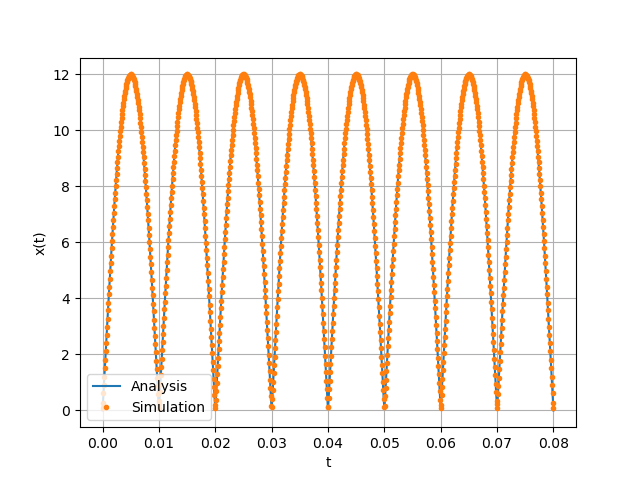
\includegraphics[width=\columnwidth]{./figs/2.3.png}
			\caption{}
			%\label{fig:ckt}
\end{figure}
         \item Show that 
    \begin{align}
        x(t) = \sum_{k = 0}^{\infty}\brak{a_k\cos{2\pi kf_0 t}+b_k\sin{2\pi kf_0 t}}
    \label{eq:one-Z-real}
    \end{align}
    and obtain the formulae for $a_k$ and $b_k$.\\
    \solution
    Using \eqref{eq:one-Z-complex},
    \begin{align}
    x(t) = \sum_{k = -\infty}^{\infty}c_ke^{j2\pi kf_0 t}
    \end{align}
    As,
    \begin{align}
    e^{j2\pi kf_0 t}=\cos\brak{2\pi kf_0 t}+j\sin\brak{2\pi kf_0 t}
    \end{align}
    From \eqref{eq:one-Z-complex}, we have,
    \begin{align}
    x(t) &= \sum_{k = -\infty}^{\infty}c_k\sbrak{\cos\brak{2\pi kf_0 t}+j\sin\brak{2\pi kf_0 t}}\\
    \label{eq:2.4}
    &=\sum_{k = -\infty}^{\infty}c_k\cos\brak{2\pi kf_0 t}+jc_k\sin\brak{2\pi kf_0 t}\\
    &=\sum_{k = -\infty}^{-1}\sbrak{c_k\cos\brak{2\pi kf_0 t}+jc_k\sin\brak{2\pi kf_0 t}} \\ &+c_0+\sum_{k = 1}^{\infty}\sbrak{c_k\cos\brak{2\pi kf_0 t}+jc_k\sin\brak{2\pi kf_0 t}}\\
    &=\sum_{k = 1}^{\infty}\sbrak{c_{-k}\cos\brak{2\pi kf_0 t}-jc_{-k}\sin\brak{2\pi kf_0 t}}\\ &+c_0+\sum_{k = 1}^{\infty}\sbrak{c_k\cos\brak{2\pi kf_0 t}+jc_k\sin\brak{2\pi kf_0 t}}\\
    &=c_0+\sum_{k = 1}^{\infty}\bigg(\brak{c_k+c_{-k}}\cos\brak{2\pi kf_0 t}\\ &+j\brak{c_k-c_{-k}}\sin\brak{2\pi kf_0 t}\bigg)
    \end{align}
    Substituting $a_k=c_{k} + c_{-k}$ and $b_k=j(c_{k}-c_{-k})$,we get,
    \begin{align}
x(t)&=c_0+    \sum_{k = 1}^{\infty}\brak{a_k\cos{2\pi kf_0 t}+b_k\sin{2\pi kf_0 t}}\\
&=\sum_{k = 0}^{\infty}\brak{a_k\cos{2\pi kf_0 t}+b_k\sin{2\pi kf_0 t}}
    \end{align}
    \begin{align}
    \label{eq:u1}
    \therefore a_k&=
    \begin{cases}
    c_k+c_{-k}&k\neq0
    \\
    c_0&k=0
    \end{cases}\\
    \label{eq:u2}
    b_k&=j\brak{c_k-c_{-k}}
    \end{align}
    Using \eqref{eq:one-Z},
    \begin{align}
    c_k &= f_0\int_{-\frac{1}{2f_0}}^{\frac{1}{2f_0}}x(t)e^{-j2\pi kf_0 t}\, dt\\
    c_{-k} &= f_0\int_{-\frac{1}{2f_0}}^{\frac{1}{2f_0}}x(t)e^{j2\pi kf_0 t}\, dt\end{align}
    \begin{align}
    a_k=c_k+c_{-k}&= f_0\int_{-\frac{1}{2f_0}}^{\frac{1}{2f_0}}x(t)\sbrak{e^{-j2\pi kf_0 t}+e^{j2\pi kf_0 t}}\, dt\\
    &=2f_0\int_{-\frac{1}{2f_0}}^{\frac{1}{2f_0}}x(t)\cos\brak{2\pi kf_0t}\, dt
    \end{align}
    Similarly, for $b_k$, we get,
    \begin{align}
    b_k=-j\cbrak{2f_0\int_{-\frac{1}{2f_0}}^{\frac{1}{2f_0}}x(t)\sin\cbrak{2\pi kf_0t}\, dt}
    \end{align}
    \item Find $a_k$ and $b_k$ for 
        \eqref{eq:x(t)}\\
        \solution
        Using \eqref{eq:u1} and \eqref{eq:u2} with \eqref{eq:ck},
    \begin{align}
    a_k&=c_k+c_{-k}=\begin{cases}
\frac{4A_0}{\pi\brak{1-k^2}}&k=even
\\
\frac{2A_0}{\pi}&k=0
\\
0&k=odd
\end{cases}\\
b_k&=j\brak{c_k-c_{-k}}=0
    \end{align}
    \item Verify 
    \eqref{eq:one-Z-real}
    using python.\\
     \solution 
        \begin{lstlisting}
wget https://github.com/Pradeep8802/EE3900-Digital-Signal-Processing/blob/main/charger/codes/2.6.py
        python3 2.3.py
        \end{lstlisting}
          \begin{figure}[!ht]
			\centering
			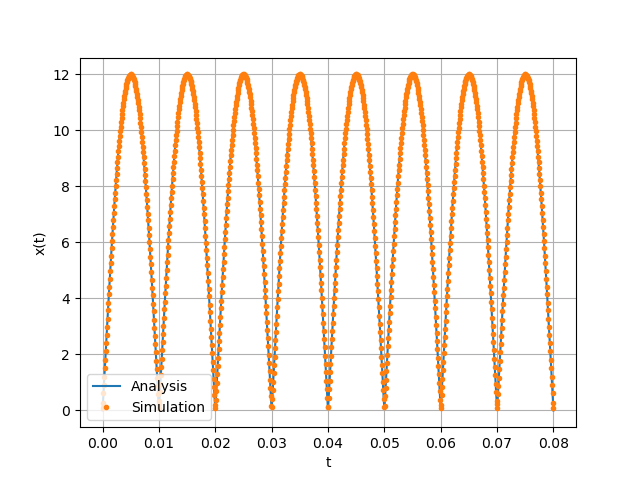
\includegraphics[width=\columnwidth]{./figs/2.6.png}
			\caption{}
			%\label{fig:ckt}
\end{figure}
    \end{enumerate}
    \end{document}